% \mysection{5}{METODOLOGÍA}
\section{METODOLOGÍA}

Para poder diseñar una arquitectura de microservicios efectiva, correcta y que responda a las
necesidades del negocio se propone una metodología iterativa que se compone de cinco etapas:


\subsection{Identificar el dominio del negocio}

Puede sonar como un axioma sin sentido, después de todo ¿qué negocio no sabe cuál es su dominio?
Sin embargo muchos arquitectos expertos siempre aconsejan empezar por aquí debido a que si bien los
expertos del dominio conocen la parte de negocio en la cual se desenvuelven, es altamente probable
que no conozcan los detalles del cómo funciona el negocio fuera de sus actividades cotidianas.

En concreto, un empleado del departamento de ventas puede conocer muy bien sus responsabilidades
y funciones dentro del flujo de ventas.
Además conoce relativamente bien las responsabilidades y funciones de los departamentos con los que más
interacción tiene (para este ejemplo almacén).
Sin embargo no conoce de los detalles de las funciones que estos otros departamentos cumplen, específicamente
no conoce de la cantidad exacta de productos que existen físicamente en almacén, no conoce los horarios
de reaprovisionamiento, no sabe que desde la semana pasada almacén tiene un nuevo vehículo que hará que
el trabajo sea más rápido.

El escenario mencionado se repite departamento a departamento, unidad de trabajo a unidad de trabajo
a lo largo y ancho de toda la organización.
Es debido a esto que es probable que la organización no tenga en claro específicamente qué acciones
son las que entregan valor y por lo tanto identificar el dominio del negocio debe ser el punto de inicio
para el equipo de desarrollo.

\subsubsection*{Entradas}
\begin{enumerate}[a.]
	\item Documentos internos de la empresa.
\end{enumerate}

\subsubsection*{Técnicas y herramientas}
\begin{enumerate}[a.]
	\item Reuniones multi-departamentales.
	\item Revisión de documentos internos.
	\item Seguimiento de flujo de producto.
\end{enumerate}

\subsubsection*{Salidas}
En esta etapa no existen salidas concretas debido a que lo único que se quiere es que el equipo
de desarrollo entienda en un nivel alto el dominio de la empresa u organización.

\subsection{Diseño Guiado por el Dominio}

En esta etapa utilizaremos las pautas que nos da el diseño basado en dominios.
Se utiliza este marco porque ya fue probado múltiples veces en el mundo real para ir desde
el nivel más alto de la aplicación hasta definir los detalles de organización de los microservicios.

Debido a que se propone una metodología iterativa para refinar los microservicios, el marco de trabajo
de diseño basado en dominios tiene la ventaja de que también está pensado como un proceso iterativo
por lo cual es congruente a la metodología propuesta.

\subsubsection{Análisis del Dominio}

El equipo de desarrollo ya tiene una idea general de qué es el dominio del negocio, pero no tiene
nada formal con lo que empezar a implementar la solución.
Entonces lo que se debe hacer es crear un modelo del dominio.
Este modelo permite ver el dominio del negocio de manera holística para poder identificar
los sub-dominios núcleo, los subdominios de soporte y los subdominios genéricos.

\subsubsection*{Entradas}
\begin{enumerate}[a.]
	\item Flujo de valor informal de la organización.
\end{enumerate}

\subsubsection*{Técnicas y herramientas}
\begin{enumerate}[a.]
	\item Event Storming
	\item Cuadros de dominios.
\end{enumerate}

\subsubsection*{Salidas}
\begin{enumerate}[a.]
    \item Sub-dominios núcleo.
    \item Sub-dominios de soporte.
    \item Sub-dominios genéricos.
\end{enumerate}

\subsubsection*{Ejemplo de la técnica event storming}


\subsubsection*{Ejemplo de la técnica cuadro de dominio}
% \imgMetodologia{cuadro_dominio}{Ejemplo de un cuadro de dominio}

  \begin{figure}[htb]
    \caption{\\\hspace{\textwidth} Ejemplo de un cuadro de dominio}
    \centering
    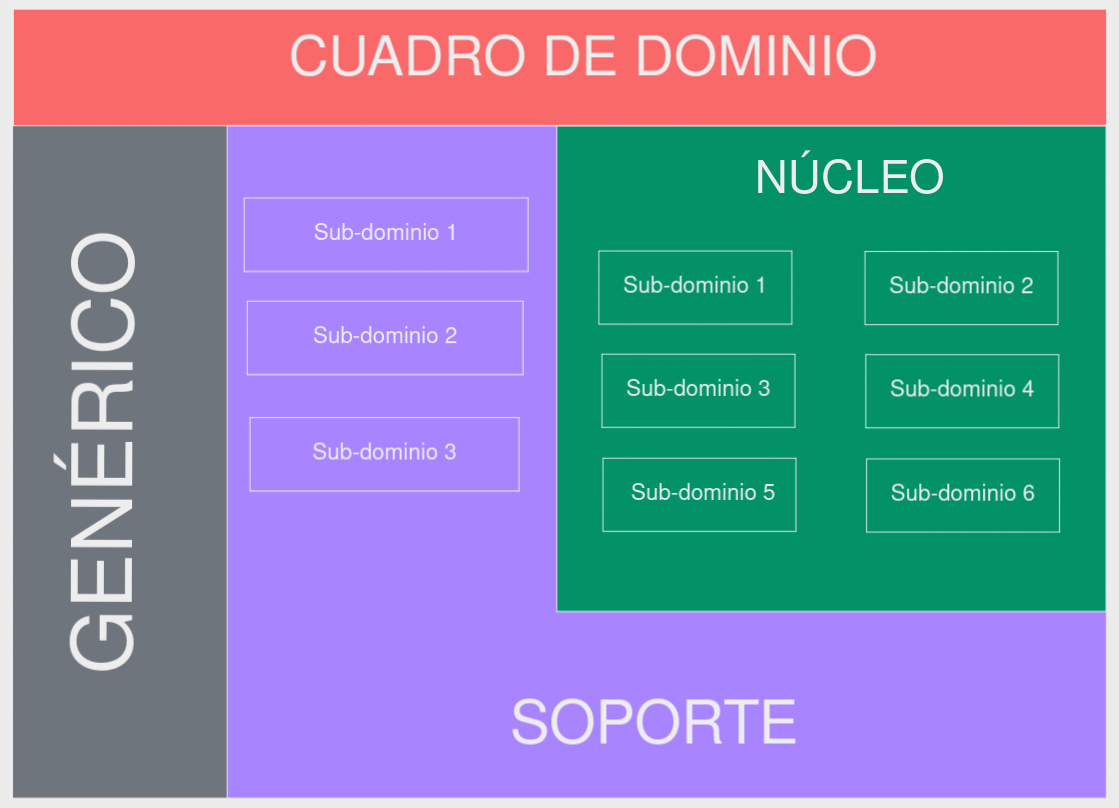
\includegraphics[width=0.90\textwidth]{src/assets/metodologia/cuadro_dominio}
  \end{figure}
\subsubsection{Definir contextos delimitados}


\subsubsection{Definir entidades, agregados y servicios}


\subsubsection{Identificar los microservicios}



Entregables propuestos para esta etapa:

\subsection{Crear un ApiGateway como punto de entrada a los servicios}

\subsection{Aseguramiento de la calidad}
